\chapter{Dise\~no}
%

\section{Dise\~no de alto nivel}
%
Lo primero a considerar es la forma de comunicaci\'on entre la computadora y
la impresora, y si bien el dise\~no debe centrarse en mantener los costos de
producci\'on y construcci\'on bajos de nada sirve un dispositivo basado en
tecnolog\'ia a en desuso o pronta a desaparecer. Es por esto que en vez de
elegir m\'etodos convencionales como lo pueden ser el protocolo serial
R232\footnote{V\'ease - \url{http://es.wikipedia.org/wiki/RS-232}} o
paralelo\footnote{V\'ease - \url{http://es.wikipedia.org/wiki/Puerto_paralelo}}
(t\'ipico de impresoras antiguas), se usar\'a el protocolo serie de
comunicaci\'on \emph{USB}\footnote{El est\'andar se explica en detalle en
\fullref{cap:usb}.} \'Este est\'andar se encuentra en la mayor\'ia de los
equipos actuales y provee una versatilidad y flexibilidad como pocos.\\

Otro tema muy importante a considerar es el sistema operativo a usar en la
computadora. Si bien puede pensarse como respuesta obvia el sistema operativo
de Microsoft,
Windows\footnote{V\'ease - \url{http://www.microsoft.com/spain/windows/}} (en
su versi\'on m\'as comercializada \emph{XP}), este enfoque fuerza al potencial
usuario a comprar una licencia\footnote{Dichas licencias rondan los 100 US\$}
solo para poder utilizar la impresora.\
Entonces en vez de optar por un sistema pago se usar\'a el sistema
operativo \emph{GNU/Linux}
% ###--->>> Poner referencia a la secci\'on donde hablo de gnu/linux
del cual existen mas de mil versiones distintas, la mayor\'a de ellas
gratuitas.
De esta forma el usuario puede obtener una copia de este sistema operativo
gratuito y usar la impresora sin mayores restricciones.\\

En la figura \ref{fig:pc_usb_printer} se muestra un esquema b\'asico de lo
dicho
anteriormente. El esquema en su m\'as alto nivel ser\'a usar una computadora
con \emph{GNU/Linux} como sistema operativo y una conexi\'on mediante
\emph{USB} al dispositivo.

\begin{figure}[htp]
\centering
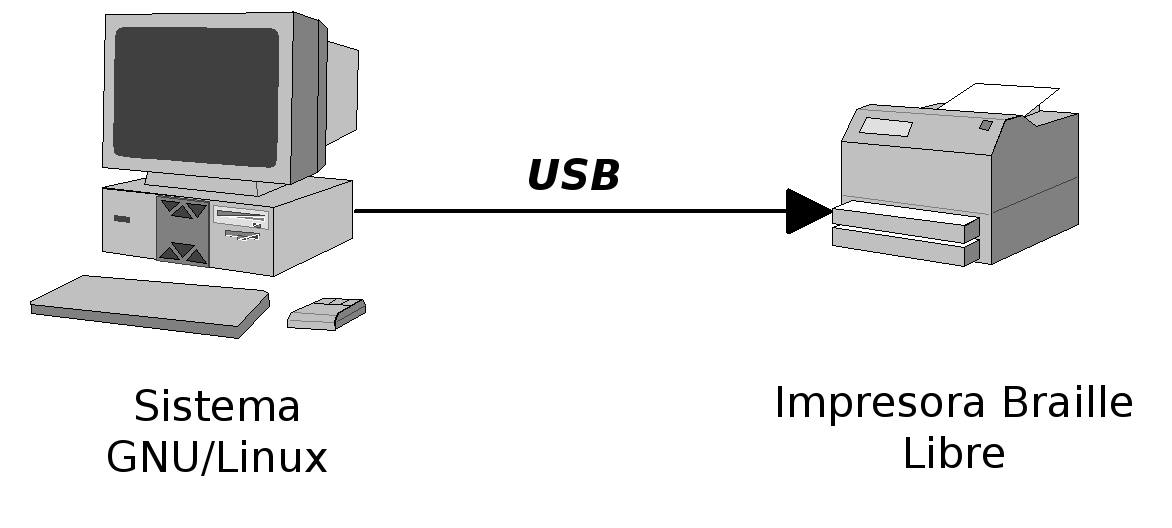
\includegraphics[width=13cm]{./img/pc_usb_printer.png}
\caption{S.O, conexi\'on e impresora}
\label{fig:pc_usb_printer}
\end{figure}

\section{Dise\~no de nivel medio}
%
Lo primero a analizar es el microcontrolador a usar. El mercado de
desarrollo electr\'onico Argentino tiene una tendencia a usar las soluciones de
Microchip\footnote{V\'ease - \url{http://www.microchip.com/}}, y es por ello
que existe mucha gente capacitada en los microcontroladores de esta empresa, y
si bien sus productos no son los mejores del mercado internacional, sus
precios son bastantes competitivos al igual que las funcionalidades que
prestan y la amplia gama de variedades que poseen.\

Como el objetivo de este trabajo se enfoca en el mercado local y el bajo costo
de producci\'on, los productos de Microchip se presentan como la mejor
alternativa.\\

El requerimiento primario para elegir el microcontrolador a usar es que posea
soporte USB. La familia \emph{18FXXXX}\footnote{V\'ease - \url{
http://www.microchip.com/stellent/idcplg?IdcService=SS_GET_PAGE&nodeId=2654}}
satisface este requerimiento. De esta familia los dos microcontroladores m\'as
comercializados\footnote{Esto implica facilidad a la hora de conseguir en el
mercado local.} en el pa\'is son el \emph{18F2550} y el \emph{18F4550}. La
tabla \ref{tab:table_12_14} muestra las principales caracter\'isticas de ambos
microcontroladores.

\begin{table}[ht]
\begin{scriptsize}
\centering
% use packages: array,booktabs
\begin{tabular*}{\textwidth}{@{\extracolsep{\fill}}|l|c|c|} \hline
 \rowcolor[gray]{.9}
 & 18F2550 & 18F4550 												\\ \hline 
 Program Memory Type & Flash & Flash								\\ \hline
 Program Memory (KB) & 32 & 32										\\ \hline
 CPU Speed (MIPS) & 12 & 12											\\ \hline
 RAM Bytes & 2048 & 2048											\\ \hline
 Data EEPROM (bytes) & 256 & 256									\\ \hline
 Digital Communication Peripherals & 1-A/E/USART, 1-MSSP(SPI/I2C) &
1-A/E/USART, 1-MSSP(SPI/I2C) 										\\ \hline
 Capture/Compare/PWM Peripherals & 2 CCP &  CCP, 1 ECCP 			\\ \hline
 Timers & 1 x 8-bit, 3 x 16-bit & 1 x 8-bit, 3 x 16-bit 			\\ \hline
 ADC & 10 ch, 10-bit & 13 ch, 10-bit								\\ \hline
 Comparators & 2 & 2 												\\ \hline
 USB (ch, speed, compliance) & 1, Full Speed, USB 2.0 & 1, Full Speed, USB 2.0
																	\\ \hline
 Temperature Range (C) & -40 to 85 & -40 to 85  					\\ \hline
 Operating Voltage Range (V) & 2 to 5.5 & 2 to 5.5					\\ \hline
 Pin Count & 28 & 40												\\ \hline
\end{tabular*}
\caption{Comparaci\'on PIC18F2550 y PIC18F4550} 
\label{tab:table_12_14}
\end{scriptsize}
\end{table}


Se observa que no existe gran diferencia entre ambos MCU\footnote{Del ingles
\emph{Micro Controller Unit}}, al igual que sus precios como se observa en la
tabla\ref{tab:table_12_14_price}.

\begin{table}[ht]
\centering
\begin{tabular}{l|r}
 \toprule
  MCU & US\$		\\ \hline
 18F2550 & 2.39  	\\ 
 18F4550 & 3.65 	\\
 \bottomrule
\end{tabular}

\begin{tiny} 
\caption{Comparaci\'on de precios PIC18F2550 y PIC18F4550}\footnote{Los precios
fueron extraidos de la p\'agina oficial de Microchip}
\end{tiny} 
\label{tab:table_12_14_price}
\end{table}




\begin{figure}[htp]
\centering
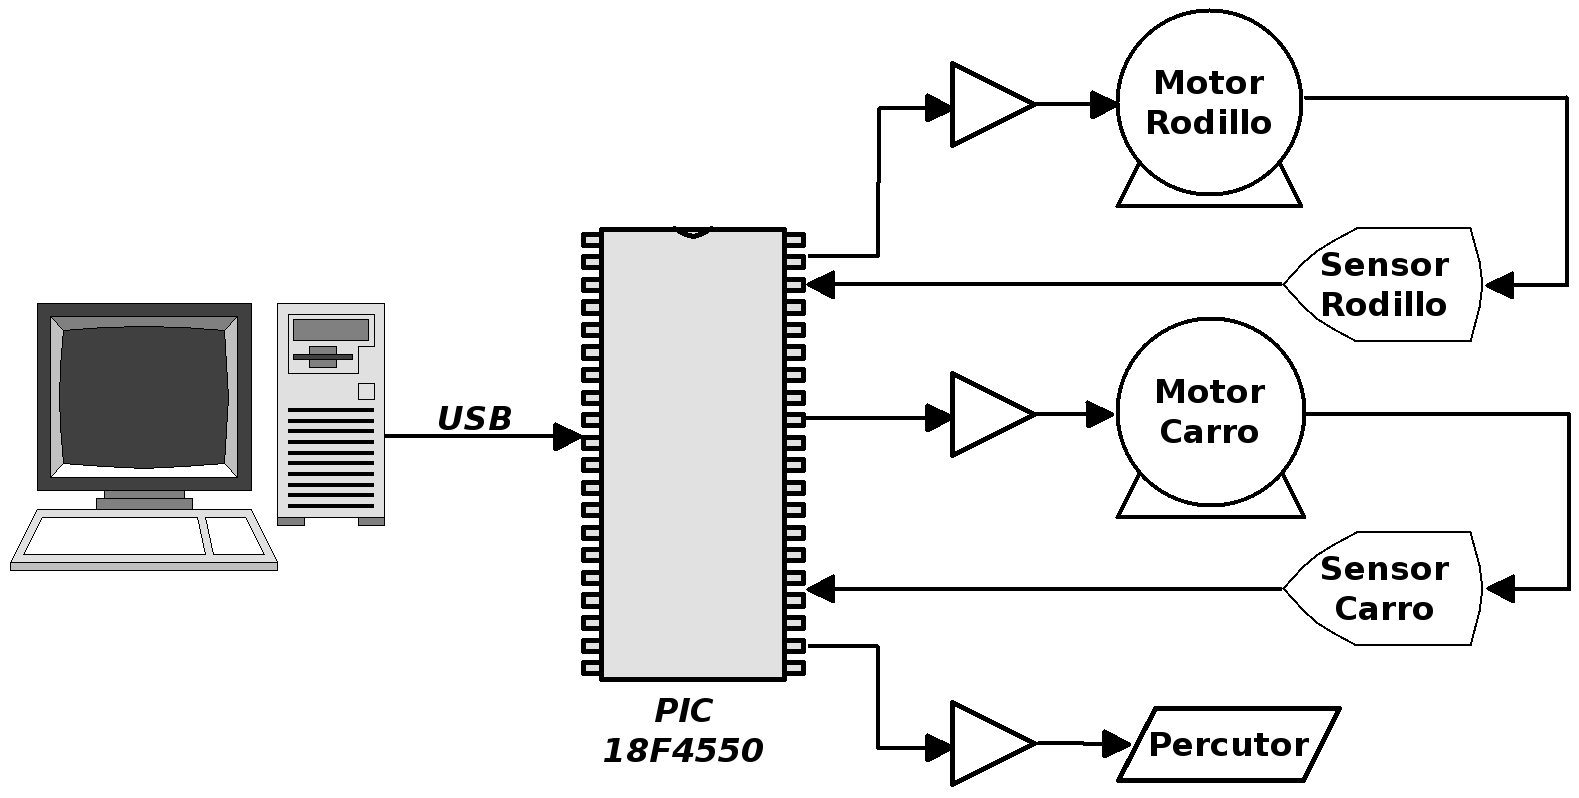
\includegraphics[width=13cm]{./img/pc_uc_motors.png}
\caption{S.O, conexi\'on e impresora}
\label{fig:pc_uc_motors}
\end{figure}